\documentclass[../main/main.tex]{subfiles}

\newdate{date}{26}{11}{2020}


\begin{document}

\chapter{Temporal Networks}

\marginpar{ \textbf{Lecture 17.} \\  \displaydate{date}. \\ Compiled:  \today.}

Let us discuss about networks that change structure in time (see Fig. \ref{fig:17_01}). This kind of networks are called \textbf{temporal networks}. There are actually many of them: for instance let us consider the \textit{face-to-face interactions} network. It is obviously a temporal network: nodes are indeed individuals and an edge is present depending on whether we are talking to each other at the considered time instant. Since one usually does not have conversations that last so much time, edges vary in time. Data for this network can be collected through \textit{RFID}: they are radio frequency detector devices than can be tuned to 1-2 meters distance. If two people come across into each other, then they send the data to a third antenna which keeps track of such contacts.
Another example of these network is the \textit{bovine displacement} among farms (see Fig. \ref{fig:17_02}) in Italy. Nodes represent farms, and every node is connected to others if cattle were sold and moved from a farm to another.

\begin{figure}[h!]
\centering
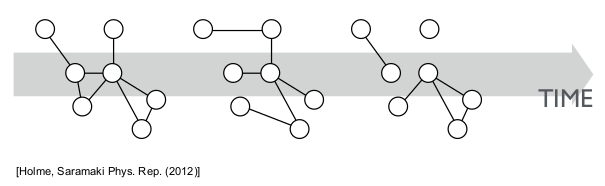
\includegraphics[width=0.5\textwidth]{../lessons/image/17/image01.png}
\caption{\label{fig:17_01} A temporal network is a network whose edges vary as time passes.}
\end{figure}


\begin{figure}[h!]
\centering
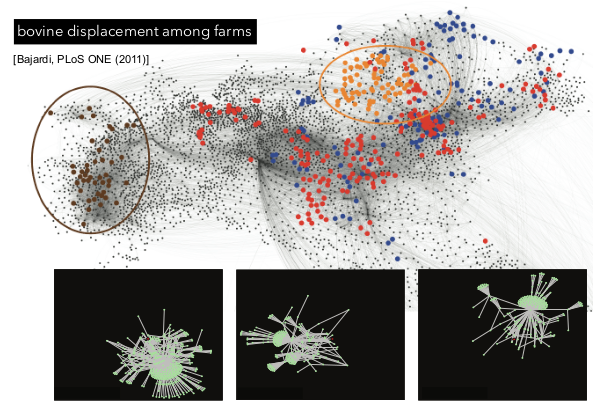
\includegraphics[width=0.65\textwidth]{../lessons/image/17/image02.png}
\caption{\label{fig:17_02} Bovine displacements among farms network. }
\end{figure}


Despite the unquestionable usefulness of such networks, there are some \textbf{issues} that arise.

The first problem regards \textbf{data visualization}. We are dealing with networks as the one in figure \ref{fig:17_03}: we treat \textit{time} as a \textit{continuous variable} and we draw \textit{edges} and see how they change. However, the \textbf{sequence of links} is not a good representation to spot communities/topology: indeed we see what happens and at what moment, but in this way it is difficult to have a general overview. It allows us to preserve the whole information but, actually, it cannot be easily analyzed. As one can imagine, we must make a choice and understand what is really important to our problem.


\begin{figure}[h!]
\centering
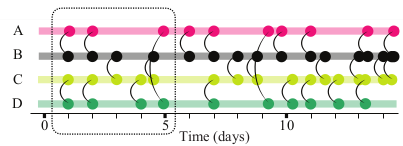
\includegraphics[width=0.9\textwidth]{../lessons/image/17/image03.png}
\caption{\label{fig:17_03} Example of temporal network using \text{sequence of links} in time representation.}
\end{figure}


Some possible \text{solutions} are the following ones and are depicted in Fig. \ref{fig:17_04}:
\begin{itemize}
    \item \textbf{aggregate} the \textbf{weights} and \text{lose time dimensionality}: the longer the time nodes are connected, the larger the weight. Building a static network makes us lose much information, however these are the simplest networks we may work with and shows clearly topology and communities;
    \item \textbf{discretize the time} that is to say \textbf{sample} the network according to rules (\textbf{daily snapshot}). This helps us thinning our network, but at the end we have still to deal with a temporal network (but discretized, so it can be seen as a set of static networks) even though a less complex one, and might lead to some misunderstanding.
\end{itemize}


\begin{figure}[h!]
\begin{minipage}[c]{0.5\linewidth}
\subfloat[][\textbf{Solution 1:} Aggregate the network as a static weighted one. Only first 5 days are considered as a time window.]{ 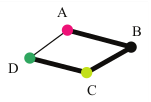
\includegraphics[width=0.8\textwidth]{../lessons/image/17/image04a.png}  \label{fig:} }
\end{minipage}
\begin{minipage}[]{0.5\linewidth}
\centering
\subfloat[][\textbf{Solution 2:} Discretize the time and sample according to some rule.]{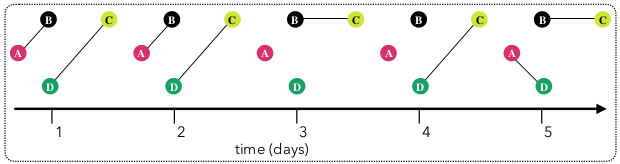
\includegraphics[width=0.8\textwidth]{../lessons/image/17/image04b.png}  \label{fig:} }
\end{minipage}
\caption{\label{fig:17_04}Possible solutions for visualization issue with temporal networks.}
\end{figure}

\marginpar{
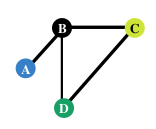
\includegraphics[width=\marginparwidth]{../lessons/image/17/image05.png}
\captionof{figure}{\label{fig:17_05} Reachability issue is not important in static networks.}
}

The second \textbf{issue} one may face when dealing with temporal network is \textbf{reachability}. We say that $i$ is \textbf{reachable} from $j$ if it exists a path $i\to j$. This is indeed a very easy problem to tackle when dealing with \textit{undirected static networks}: every node belonging to the same \textbf{connected component} is reachable from the other members. On the other hand, if the network where we start from is a temporal one, a static network might be the output we obtain after aggregating it. However in this we are losing some important information: if, for instance, two nodes share a link only at the very beginning, we see them as connected even though they are not present any more after a certain time instant. It actually shows lots of path that might be \textbf{not} available any more. Hence, the \textbf{existence} of a \textit{time respecting path} does depend on the window $[t,T]$ of observation (see fig. \ref{fig:17:07a})!

As said, in an \textbf{undirected temporal network}, $j$ is reachable from $i$ only if there exist a \textbf{time respecting patch} $i \to j$. That is to say that there is a \textbf{sequence of contacts} that connects $i \to j$ with each contact in the path coming sequentially one after the other from node $i\to j$ (see Fig. \ref{fig:17_06}).

\begin{figure}[h!]
\centering
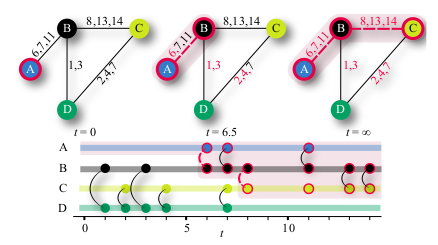
\includegraphics[width=0.7\textwidth]{../lessons/image/17/image06.png}
\caption{\label{fig:17_06} The existence of temporal paths between two nodes depends on time. }
\end{figure}


\begin{figure}[h!]
\begin{minipage}[c]{0.5\linewidth}
\subfloat[][Reachability depends on the choice of time window.]{ 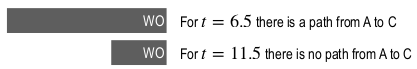
\includegraphics[width=0.8\textwidth]{../lessons/image/17/image07a.png}  \label{fig:17:07a} }
\end{minipage}
\begin{minipage}[]{0.5\linewidth}
\centering
\subfloat[][Whether infection spreads depends both on the disease, in particular $\mu$, and on the time window.]{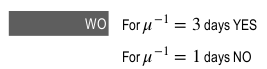
\includegraphics[width=0.8\textwidth]{../lessons/image/17/image07b.png}  \label{fig:} }
\end{minipage}
\caption{\label{fig:} }
\end{figure}


One should recall that we are dealing with \textbf{epidemic spreading}: if we aggregate network into a static one, possibilities to infect other nodes are much larger rather then what happens for temporal network.  Moreover, infection has a certain duration that is given by the \textbf{recovery rate} $\mu$: the longer it is, the more likely we stay infected and are able to infect other nodes spreading the disease. On the other hand, when infection duration is small we may recover without having the time to spread it to other nodes that at that moment are not connected to us (see fig. \ref{fig:17:07b}).


The third \textbf{issue} that arises is the \textit{activation frequency} or, in other words, the \textbf{contact heterogeneities}. In static network, we know that there are actually some nodes that have more contacts whereas some have few. The analogous for temporal networks is that, besides the \textit{number of contacts} a node may have, we must consider how \textbf{often activation occurs}.
That is to say: if a node activates often and has many contacts, for sure it will lead to a different spreading rather than a node that activates less often and has few contacts. It is also different in terms of epidemic spreading if, once fixed the number of contacts, we have them as "one-shot" (we go to a party and meet lot of people) or diluted wrt time (daily we meet few people): at the end the number of total contacts will be the same. Indeed, the \textbf{cumulative number of contacts} results from \textit{activation frequency} and \textit{number of contacts per activation}.


Another \textbf{issue} we have to tackle is the \textbf{non homogeneous activation}, that is to say that \textbf{inter-contact} times (i.e. \textit{inter-occurence} time) between activations is not exponential and the number of contacts cannot be modeled as Poisson. Therefore, individuals do not have some sort of general \textit{activation rate}: it is a more complex process, since according to an exponential distribution longer periods are not allowed (see fig.\ref{fig:17_08}). Indeed, empirical data suggests us that human behavior is \textbf{bursty}, and this \textit{burstiness} is reflected in broader-than-expected distribution of inter-contact times. Some datasets, for example face-to-face interactions, emails, or phone calls suggested that the best model that reflects human social activity is a power law with a cutoff:
\begin{equation*}
    P_{E} ( \tau ) = A \tau ^{-\alpha} e^{-\tau/\tau_E}
\end{equation*}
Indeed, we usually stay inactive for a while, and then have a burst: we start reply to just received messages and eventually start a conversation (\textit{causality effect}).

\begin{figure}[h!]
\centering
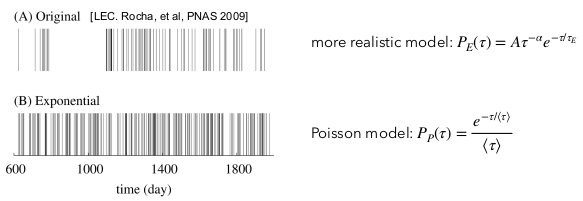
\includegraphics[width=0.9\textwidth]{../lessons/image/17/image08.png}
\caption{\label{fig:17_08} Inter-contact times can be modeled according different distributions, which lead to very different behaviors. }
\end{figure}

The last \textbf{issue} is the most complex one to be captured by models and involves \textbf{temporal correlations}. Every time a node activates, there is the chance that the \textbf{contacts} it makes are \textbf{correlated} to the contacts it had in the \textbf{past}. A possible workaround is to introduce the so called \textbf{social strategy}\footnote{Miritello, et al, Sci Rep 2013.}:
\begin{equation}
    \gamma_{i,t} = \frac{k_{i,t}}{s_{i,t}}
\end{equation}
where $k_{i,t}$ and $s_{i,t}$ are respectively the \textit{degree} and the \textit{weighted degree} of $i$ in the network aggregated over the interval $[t-\delta, t]$. For $\gamma \to 0$ we have a \textit{memory-driven behavior}, so a node tends to make contacts always with the same nodes (social keeper), while for $\gamma \to 1$ the behavior is memoryless, therefore a node shows a more socially exploratory behavior.





\section{Temporal networks dynamics}

Let us consider now, once we have a dataset with temporal description of the network, how its main \textbf{properties affect} the \textbf{dynamics}. Up to some years ago, temporal networks were not considered of much interest: for instance indeed under some assumption, namely the \textbf{time scales separation}, the time dimension seemed not to be relevant in the spreading process and therefore was dropped.

Let us refer to the \textbf{average infectious duration} with $\mu^{-1}$, while let $\tau$ be the \textbf{average contact time}. For $\tau \ll \mu^{-1}$ we do not need to take into account contacts with a high resolution in time, being the network faster than the disease: considering the average network would be actually sufficient. Conversely, if the network is slower than the disease (e.g. migration network), namely $ \tau \gg \mu^{-1} $, one may want to exploit the static network and drop the time information. We want to understand when $\tau \sim \mu^{-1}$, so when \textbf{timescales} are \textbf{comparable}. This can be done obviously if and only if \textbf{timescales are definite}: there might be some distributions whose mean is not informative, since its variance is high and a timescale cannot be defined out of them.

We can follow two main approaches when dealing with temporal networks in epidemiology: \textbf{bottom-up} perspective and \textbf{top-down} approaches.
In the first one, we start \textit{building mathematical} models for human interactions and the spreading dynamics. However, this is not at all a simple approach and requires too much work. The second approach is to take some \textit{empirical networks} and \textit{run numerical simulations} over them, by randomising (i.e. neglecting/throwing away) some properties whose we want to study the effects. In this way, we are able to understand the \textit{impact of a specific property} in the spreading process.



\subsection{Activity driven model}

It is the first and the simplest model\footnote{Perra et al, Sci Rep 2012.} that was introduced to study human interactions, where nodes activate according to a certain rate. It follows the so-called \textbf{bottom-up} approach.

\marginpar{
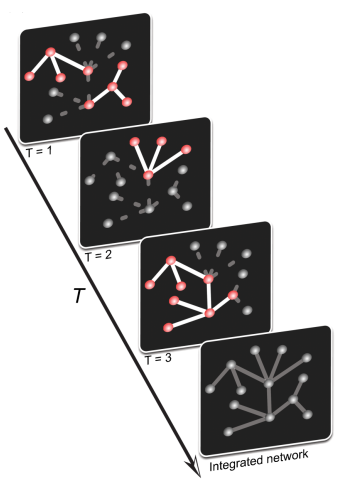
\includegraphics[width=\marginparwidth]{../lessons/image/17/image09.png}
\captionof{figure}{\label{fig:17_09} Activity driven model.}
}

The main \textbf{ingredients} for this model are:
\begin{itemize}
    \item $\Delta t$ timestep, indeed time is discretized;
    \item $N$: number of nodes;
    \item $x_i$: activity potential, that is the number of activations of $i$ during $\Delta t$ and is normalized over the total number of activations $(\varepsilon \leqslant x_i \leqslant 1)$;
    \item $F(x)$: distribution of the activity potential;
    \item $a_i = \eta x_i$ activation rate, where $\eta$ is a rescaling factor chosen to tune the average number of active nodes per unit time in the system $\bar{N} = \eta\expval{x}N$;
    \item $m$: number of connections made at each activation, it is the same for all the nodes.
\end{itemize}
The \textbf{algorithm} for the model is indeed the following:
\begin{itemize}
    \item at each time step $t$ the network $G_t$ starts with $N$ nodes that are \textit{all} disconnected;
    \item node $i$ activates with probability $a_i \Delta t$ and makes $m$ links with other randomly selected nodes. Non-active nodes are still able to receive connections from active nodes;
    \item at the next time step $t + \Delta t$ all the edges are deleted, so all links last $\tau_i = \Delta t$.
\end{itemize}
This model actually captures the issue introduced when talking about \textbf{heterogeinity in activations}: now we are indeed modelling Poisson activations, despite the rate of activation is heterogeneous.
In addition, it does not take into account possible correlations between activations.
Moreover, \textit{network at each timestep} has \textit{on average} $E_t = m \eta \expval{x} N$ \textbf{edges} and $\expval{k}_t = \frac{2E_t}{N} = 2 m \eta \expval{x}$ \textbf{average degree}. At the end of the day the \textbf{topology} of the network is \textit{homogeneous}\footnote{$P(k)$ is Poisson}, even though \textbf{activation rate} is \textit{heterogeneous}!


Now we want to understand how properties change when we \textbf{integrate the network over a time window} $T$. The \textbf{degree} of a node $i$, in the aggregated network is:
\begin{equation}
    k_T(i) = k_T^{OUT} (i) + k_T^{IN}(i)
\end{equation}

Let us focus on the first term \( k_T^{OUT} (i) \): $i$ makes on average $T a_i m$ links.
We want to understand how many different nodes $i$ connects to, without counting twice repeated links with the same node. This should resemble the \textit{Urn problem}, where we want to count the number of \textit{different} balls extracted from an urn with $N$ balls after $T$ extractions.
We know that the probability for each ball (node) to be extracted at least once is $p = 1 - \qty[ 1 - 1/N ]^{T a_i m}$ and the probability of extracting $d$ balls is binomial with parameters $\text{Bin}(p, N, d)$. Hence, the average number of balls $k_T^{OUT}$ is:
\begin{equation}
    \expval{ k_T^{OUT} } = Np = N [1-e^{-\frac{T a_i m}{N}} ]
\end{equation}
as $N \to \infty$ and the time window is such that $T/N \to 0$.


Let us focus on the other term $k_T^{IN}(i)$, that is the number of nodes that make connections with $i$ among those that were not targeted by $i$. In this way we avoid double counting. The probability that a node was not a target of $i$ is the complementary as before, that is: $[1-1/N]^{T a_i m} \sim e^{-\frac{T a_i m}{N}}$. Given that the average number of edges formed at each timestep is $m N \expval{a}$ and they can connect to node $i$ with probability $1/N$, we have that:
\begin{equation}
    \expval{k_T^{IN}} = \frac{m \cancel{N}\expval{a}}{\cancel{N}} e^{-\frac{T a_i m}{N}} = m \expval{a} e^{-\frac{T a_i m}{N}}
\end{equation}
Therefore, the degree formula can be written as function of each activity potential $a_i$:
\begin{align}
    k_T(i) = N[1-e^{-\frac{T a_i m}{N}}]
    + m \expval{a} e^{-\frac{T a_i m}{N}}
    \simeq N[1-e^{-\frac{T a_i m}{N}}]
     = N[1-e^{-\frac{T \eta x_i m}{N}}]
\end{align}
where we assumed that $N \to \infty$ and $T/N \to 0$.



Rewriting now the \textbf{activity potential} as a function of the \textit{degree} $x(k)$:
\begin{equation*}
    x(k) = - \frac{N}{\eta m T} ln\left( 1 - \frac{k}{N} \right)
\end{equation*}
We can revert both the latter formula and $P_T(k) \d{k} \sim F(x) \d{x}$, thus obtaining \textbf{degree distribution} of the aggregated network for observation in window of length $T$:
\begin{equation*}
    P_T(k) \sim F[x(k)] \dv{x(k)}{k} = \frac{1}{Tm\eta} \frac{1}{1-k/N} F\left[- \frac{N}{\eta m T} ln\left( 1 - \frac{k}{N} \right) \right]
\end{equation*}
If the time window dimension is small, namely $T\to 0$, then also $k/N \to 0$, and the latter expression can be further approximated as:
    \begin{empheq}[box=\myyellowbox]{equation}
        P_T(k) \sim \frac{1}{T m \eta} F \left[ \frac{k}{Tm\eta} \right]
    \end{empheq}
This implies that \textbf{nodes activate and form a heterogeneous network} despite they activate heterogeneously.
In other words, heterogenous topology in the \textbf{aggregated} network (i.e. there are hubs), over a window $T$, results from a heterogeneous activity potential (i.e. they activate more often). To avoid any further confusion: at each \textit{timestep} the static network is homogeneous, regardless the the activation rate which is heterogeneous. On the other hand the \textit{aggregated} network results being heterogeneous, thanks to the heterogeneous firing rate distribution.


Let us try to understand what are the \textbf{effects} on the network dynamics on epidemic spreading. For instance, let us consider how the \textbf{epidemic threshold} changes according to the activation dynamics.
In order to pursue our goal, let us use the \textbf{activity block approximation} that works as the same way as the \textit{degree block approximation}, and consider a $SIR$ model.
Let us define the \textit{probability of transmission per contact} as $\beta$, moreover let us assume $m=1$: every time a node activates, it makes a single connection. The $SIR$ equation, classifying nodes according their activity, for infected nodes at time $t + \Delta t$ within class $a$ is:
\begin{equation}
   I_a^{t+\Delta t} = -\mu \Delta t I^t_a + I^t_a + \mathcolorbox{green!20}{\beta(N_a^t - I_a^t) a \Delta t \int da' \frac{I_{a'}^t}{N} } +  \mathcolorbox{blue!20}{\beta (N_a^t - I_a^t)\int da' \frac{I_{a'}^t a' \Delta  t}{N}}
\end{equation}
The \textit{green} term describes the probability for a node in class $a$ to activate and get in contact with infected nodes of any other classes $a'$, from which it contracts the disease. The blue term, on the other hand, returns the probability we have to be infected by other infectious nodes that instead activate while we do not.
Defining the last integral $\theta^t = \int da' \frac{I_a'^t a' \Delta  t}{N} $, we are able to write the \textbf{total number of infectious} as:
\begin{equation}
    \int da I_a^{t + \Delta t} = I^{t + \Delta t} = I^t - \mu \Delta t I^t + \beta \expval{a} I^t \Delta t + \beta \theta^t \Delta t
\end{equation}
Multiplying both rhs and lhs of the last equation by $a$ and integrating over the latter, we obtain:
\begin{equation}
    \theta^{t + \Delta t} = \theta^{t} - \mu \theta^t \Delta t + \beta \expval{a^2} I^t \Delta t + \beta \expval{a} \theta^t \Delta t
\end{equation}
Up so far, we obtained two equations in two variables $I$ and $\theta$. Rewriting them as differential equations:
\begin{subequations}
\begin{align}
    \partial_t I &= -\mu I + \beta \expval{a} I + \beta \theta\\
    \partial_t \theta &= -\mu \theta + \beta \expval{a^2}I + \beta \expval{a}\theta
\end{align}
\end{subequations}

Let us understand now when these expressions return as a growth in the number of infectious. The tool we will use is \textbf{linear stability analysis}. The Jacobian is:
\begin{equation}
    J =
    \begin{vmatrix}
    -\mu + \beta \expval{a} & \beta \\
    \beta \expval{a^2} & - \mu + \beta \expval{a}
    \end{vmatrix}
\end{equation}
whose set of eigenvalues is $\Lambda_{1,2} = \beta\expval{a} - \mu \pm \beta \sqrt{\expval{a^2}}$.
We want the \textit{largest eigenvalue} to be \textbf{positive}, in order to have the number of infectious growing.

The condition for the \textit{largest eigenvalue} to be \textit{positive} is thus:
\begin{empheq}[box=\myyellowbox]{equation}
\frac{\beta}{\mu} > \frac{1}{\expval{a} + \sqrt{\expval{a^2}}} + \mathcal{O}\left(\frac{1}{N}\right)
\end{empheq}
and it sets a threshold for $\beta$ that is function of the moments of the activity distribution. Note as if activity distribution is heterogeneous, then its variance becomes large and the threshold decreases, hence favoring the spread.


Summarizing, the \textbf{activity driven model} captures the realistic property of human behavior (face-to-face, sexual contacts, phone call, email, tweets) and takes into account heterogeneous activity rate. Moreover, the contact network at a \textbf{given instant} is \textit{sparse} and has homogeneous degree. Once again, we want to stress that the \textbf{aggregated network} over a certain time window is really resembling a \textit{heterogeneous degree} network!

So if  we do not make any assumption on the pattern of activation that may unfold at the same time scale of the spreading process, computations are made possible within the \textit{activity-block} approximation, which follows the same scheme as the degree-block approximation. In conclusion, \textbf{contact heterogeneity lowers the epidemic threshold}.



\subsection{Randomised Reference Models}

Let us now discuss an example of the other type of approaches one may want to use when dealing with \textit{temporal networks}: \textbf{top-down} approaches\footnote{Gauvin et al Sci Rep 2013.}.
Let us recall we want to understand how the \textbf{temporal structure} of the network \textbf{impacts} the \textbf{spreading}. We therefore compare the epidemics on real data with the outcome in suitable null models that randomize (i.e. destroy) some properties over some others. However, we keep the topology of the aggregated network fixed.

We are going to study 3 different types of randomizations.
Let us define the following quantities:
\begin{itemize}
    \item $P(\tau)$: inter-contact time distribution;
    \item $\omega_{AB}$: cumulated contact durations of an arbitrary link $AB$;
    \item $P(\omega)$: distribution of the cumulated contacts duration;
    \item $n_{AB}$: number of contacts per link of an arbitrary link. These are the total times A, B are in contact, regardless of how much;
    \item $P(n)$ distribution of the number of contacts per link.
\end{itemize}


\begin{figure}[h!]
\begin{minipage}[c]{0.5\linewidth}
\subfloat[][Initial condition.]{ 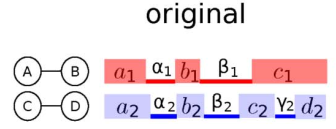
\includegraphics[width=0.8\textwidth]{../lessons/image/17/image10.png}  \label{fig:} }
\end{minipage}
\begin{minipage}[]{0.5\linewidth}
\centering
\subfloat[][IS: Interval shuffling applied.]{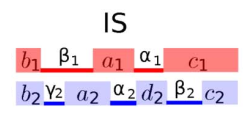
\includegraphics[width=0.8\textwidth]{../lessons/image/17/image11.png}  \label{fig:} }
\end{minipage}\\
\begin{minipage}[c]{0.5\linewidth}
\subfloat[][LS: Link Shuffling applied.]{ 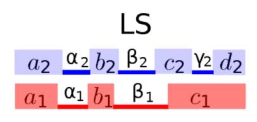
\includegraphics[width=0.8\textwidth]{../lessons/image/17/image12.png}  \label{fig:} }
\end{minipage}
\begin{minipage}[]{0.5\linewidth}
\centering
\subfloat[][GTS: Global Time Shuffling applied.]{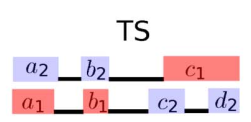
\includegraphics[width=0.8\textwidth]{../lessons/image/17/image13.png}  \label{fig:} }
\end{minipage}
\caption{\label{fig:17_15} Red (light) segments indicate $A–B$ contacts, while blue (dark) segments indicate $C–D$ contacts. For each link, individual contact intervals are marked with latin letters and inter-contact intervals with greek letters. }
\end{figure}


Let us discuss the three different of shuffling (see Fig. \ref{fig:17_15}) we may have:
\begin{itemize}
    \item \textbf{Interval Shuffling}: the sequences of contact and inter-contact durations are reshuffled for each link separately. The only property we destroy is the \textit{causality}: correlations between historical information of link are destroyed, since their chronological order (sequence) is randomized.
    \item \textbf{Link Shuffling}: the unaltered sequence of events (i.e. contacts) are swapped between link pairs. In this case we are destroying \textit{causality}: by reshuffling links we destroy causal correlations between pair nodes. Moreover, we are also dropping $\omega_{AB}$ and $n_{AB}$, since we are assigning to each link a history that has been taken randomly from other nodes. We are destroying the exact structure of the networks, i.e. swapping labels.
    \item \textbf{Global Time Shuffling}:  we build a global list of the empirical contact durations and, for each link, we generate a synthetic activity timeline by sampling with replacement the global list of contact durations according to the original number of contacts for that link. We are preserving by construction the topology, the number of connections between each pair and their distribution. On the other hand, we are destroying the remaining ones: namely \textit{causality}, $P(\omega)$, $\omega_{AB}$, $P(\tau)$ since now we are drawing randomly activation times.
\end{itemize}
See Fig. \ref{fig:17_14} in which the main shuffling characteristics are summarized.

\begin{figure}[h!]
\centering
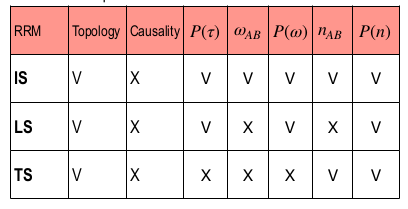
\includegraphics[width=0.9\textwidth]{../lessons/image/17/image14.png}
\caption{\label{fig:17_14} Table depicting all different types of randomizations and what property we drop. }
\end{figure}

Comparing the empirical data and the other to the ones we obtain by using the aforementioned shuffles, we are able to understand what are the \textbf{main features} of our network. In addition, we can see how these either enhance or contrast the spreading of a disease. For instance, if we destroy a property and we note that spread does not strongly change, we are even allowed to not collect data related to that property any more, thus saving time, memory and resources. On the other hand, if after shuffling it strongly changes, then we can conclude that that property plays an important role in the spread process.



\end{document}
